\documentclass[12pt]{article}

\newcommand{\cnum}{\textbf{What's Cooking?}}
\newcommand{\ctitle}[3]{\title{\vspace{-0.5in}\cnum\\#2\vspace{-1ex}}}
\usepackage{enumitem}
\usepackage{amsmath}
\usepackage[usenames,dvipsnames,svgnames,table,hyperref]{xcolor}
\usepackage{titlesec}
\usepackage{graphicx}
\usepackage[hang,flushmargin,bottom]{footmisc}
\usepackage{float}
\restylefloat{table}
\graphicspath{ {figures/} }

\setlength{\footnotemargin}{3mm}
\setlength{\skip\footins}{0.5cm}
\setlength{\footnotesep}{0.3cm}

\renewcommand*{\theenumi}{\alph{enumi}}
\renewcommand*\labelenumi{(\theenumi)}
\renewcommand*{\theenumii}{\roman{enumii}}
\renewcommand*\labelenumii{\theenumii.}


\begin{document}
\ctitle{0}{Machine Learning Engineer Nanodegree Capstone Project}{}
\author{Albert Pan}
\date{\vspace{-2ex}November 23, 2018}
\maketitle

\section{Definition}
\subsection{Project Overview}

Food plays a major part in any culture around the world. In fact, the geographical characteristics and cultural associations of a region directly influence their cuisines. By investigating the ingredients used in various cuisines, we can gain a better understanding of the geographical and cultural landscape of different regions.

Han Su et. al.\footnote{Su, Han \& Lin, Ting-Wei \& Li, C.-T \& Shan, Man-Kwan \& Chang, Janet. (2014). Automatic recipe cuisine classification by ingredients. UbiComp 2014 - Adjunct Proceedings of the 2014 ACM International Joint Conference on Pervasive and Ubiquitous Computing. 565-570. 10.1145/2638728.2641335.} has worked on investigating if recipe cuisines could be identified by their ingredients, using data from food.com. They treated each ingredient as a feature and examined the common ingredients for each cuisine. Their study provides good insight on how to approach this project and what results we could expect to achieve.

For this project, we can use machine learning techniques to attain useful predictions with our data. This project will give me an opportunity to work with real-world datasets and to learn about the relation between ingredients and cuisines. This kind of research can be expanded to other fields of study involving text classification.

\subsection{Problem Statement}
Using the data provided by Yummly\footnote{https://www.kaggle.com/c/whats-cooking-kernels-only/data}, the challenge is to predict the cuisine of the dish from its list of ingredients. More specifically, this would be multi-class classfication problem, as we have 20 different cuisines we can predict. We can use a machine learning model that utilizes this data to predict the appropriate cuisine.
\newline
\newline
%
My strategy for solving this problem is as follows:
\begin{enumerate}[label*=\arabic*.]
\item Download data from Kaggle
\item Explore data with visualizations
\item Preprocess data and extract features
\item Train and test model
\item Tune hyperparameters
\end{enumerate}

\subsection{Metrics}
As previously mentioned, our training data seems to be unbalanced, and thus I will be using the $F_1$-score to evaluate the model. The $F_1$-score is the weighted average of the precision and recall, and can be expressed mathematically with the following form:

\begin{equation}
F_1 = 2 \cdot \frac{precision \cdot recall}{precision+recall}
\end{equation}
%
We can also take a look at the precision and recall metrics on their own. Precision can be expressed with the following equation, where $dish_x$ is a dish of a particular cuisine $x$:

\begin{equation}
precision = \frac{\textit{$dish_x\: correct$}}{\textit{$total\: dish_x$}}
\end{equation}
%
where $dish_x\: correct$ is the number of dishes of cuisine $x$ that are correctly classified as $x$, and $total\: dish_x$ is the the total number of dishes that were classified as $x$.
\newline
\newline
%
Recall can expressed with:

\begin{equation}
recall = \frac{\textit{$dish_x\: correct$}}{\textit{$dish_x\: correct$} + \textit{$dish_x\: incorrect$}}
\end{equation}
%
where $dish_x\: correct$ is the number of dishes of cuisine $x$ that are correctly classified as $x$, and $dish_x\: incorrect$ is the number of dishes of cuisine $x$ that are incorrectly classified.

\section{Analysis}
\subsection{Data Exploration}
The dataset that I will be using is provided by Yummly, and it consists of two JSON files. The most important file is the \textit{train.json} file, which has 39774 rows of data, and this is the data that we will be using to train our model. The \textit{test.json} file has 9944 rows of data, and this is the data that we will be using to evaluate our model.

\begin{table}[H]
\begin{tabular}{|l|l|l|}
\hline
\textbf{id} & \textbf{cuisine} & \textbf{ingredients}                                     \\ \hline
10259       & greek            & {[}romaine lettuce, black olives, grape tomatoes, ...{]} \\ \hline
22213       & indian           & {[}water, vegetable oil, wheat, salt{]}                  \\ \hline
12734       & italian          & {[}chopped tomatoes, fresh basil, garlic, ...{]}         \\ \hline
41995       & mexican          & {[}ground cinnamon, fresh cilantro, chili powder, ...{]} \\ \hline
2941        & thai             & {[}sugar, hot chili, asian fish sauce, lime juice{]}     \\ \hline
\end{tabular}
\caption{A few examples from our training dataset.}
\end{table}

\noindent
The training data contains three fields, \textit{id}, \textit{cuisine}, and \textit{ingredients}. The \textit{id} field is a unique integer identifier for a particular dish, and is not needed for modeling or analysis. The other two fields, \textit{cuisine} and \textit{ingredients}  are very important. \textit{ingredients} consists of the list of ingredients for each dish, while \textit{cuisine} denotes the cuisine. We will be extracting our features from \textit{ingredients} and we will be trying to predict the target class \textit{cuisine}.

\subsection{Exploratory Visualization}

To better understand the data, we can take a look at the distribution of cuisines in our training data:

\begin{figure}[!h]
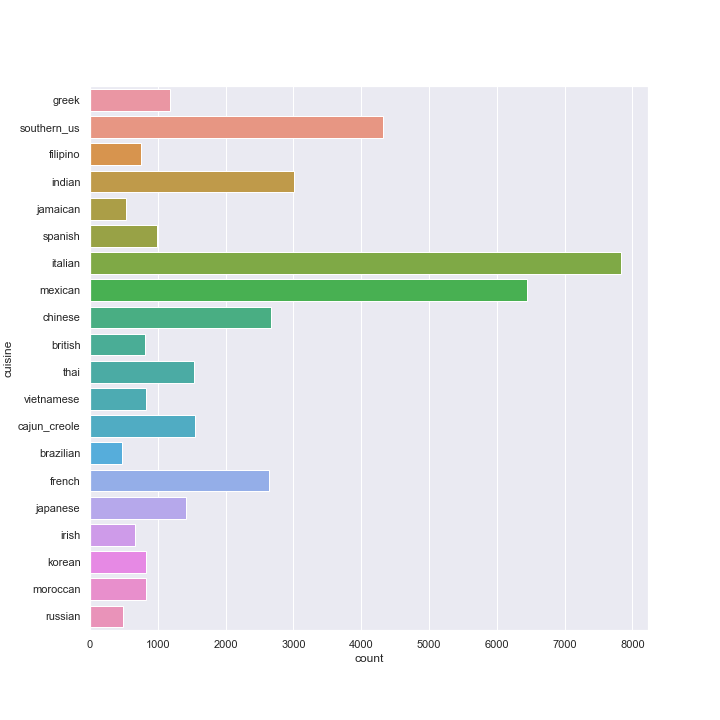
\includegraphics[width=\textwidth, height=15cm]{cuisine-distribution.png}
\caption{Cuisine distribution in training dataset}
\end{figure}

\noindent
We see that our training data is unbalanced, as there are much more "italian" and "mexican" cuisines that any of the other cuisines. This is why we decided to use the $F_1$-score as our evaluation metric, as the $F_1$-score will take into account both precision and recall.

We can also take a closer look at our ingredients. We have 6714 kinds of distinct ingredients, and a good number of them are common to different recipes and cuisines.

\subsection{Algorithms and Techniques}
This is a classification problem, and so I will be using algorithms and techniques that are suited for classification problems. In particular, I will be using the following models/algorithms:

\begin{itemize}
	\item Support Vector Machines (LinearSVC\footnote{https://scikit-learn.org/stable/modules/generated/sklearn.svm.SVC.html}): Support vector machines, or SVMs, are a set of supervised learning models that uses decision boundaries for both classification and regressions problems. SVMs construct a hyperplane that allows us to linearly separate data by transforming the feature space. For this problem, I decided to use a linear kernel because it is less computationally expensive and allows us to use multi-class classification.
	\item Naive Bayes (MultinomialNB\footnote{https://scikit-learn.org/stable/modules/generated/sklearn.naive\_bayes.MultinomialNB.html}): Naive Bayes is a supervised learning algorithm that is based on Bayes' Theorem\footnote{https://en.wikipedia.org/wiki/Bayes\%27\_theorem}, and it assumes that all of the features are independent. This particular algorithm has been historically used for SPAM detection for its speed and accuracy. For our problem, we will be using MultinomialNB (Multinomial Naive Bayes model), which is a multi-class classifier implementation of Naive Bayes.
	\item Decision Trees (DecisionTreeClassifier\footnote{https://scikit-learn.org/stable/modules/generated/sklearn.tree.DecisionTreeClassifier.html}): Decision Trees learn decision rules and generates trees that can be used for both classification and regression problems. Using the input features, it can decide which subtree to follow until it reaches the bottom of the tree, in which it will return its prediction. We will be using the DecisionTreeClassifier from the \textit{scikit-learn} library to perform multi-class classification.
	\item Random Forests (RandomForestClassifier\footnote{https://scikit-learn.org/stable/modules/generated/sklearn.ensemble.RandomForestClassifier.html}): Random forests are ensemble methods that can used to build models for classification and regression models\footnote{https://en.wikipedia.org/wiki/Random\_forest}. They operate by constructing a series of decision trees and outputting a combined prediction from all of the trees. Random Forests aim to correct the decision tree's tendency to overfit to the training data. We will be using the RandomForestClassifier, which is capable of multi-class classification.
	\item Gradient Boosted Trees (XGBClassifier \footnote{https://xgboost.readthedocs.io/en/latest/python/python\_api.html}): Gradient boosting is a technique used in both classification and regression problems. and it builds a prediction model by creating an ensemble of weak learners, usually with decision trees\footnote{https://xgboost.readthedocs.io/en/latest/tutorials/model.html}. It builds the model by utilizing the optimization of an arbitrary differentiable loss function. We will be using XGBClassifier from the \textit{xgboost} library.
\end{itemize}

\subsection{Benchmark}
For our baseline benchmark, we can use the metric obtained by predicting the most common cuisine in the training and testing datasets. The most common cuisine is \textit{Italian}, and our benchmark model will predict Italian to all recipes. This would give us a benchmark $F_1$-score of $0.3292$.

\section{Methodology}
\subsection{Data Preprocessing}

\subsection{Implementation}

\subsection{Refinement}

\section{Results}
\subsection{Model Evaluation and Validation}

\subsection{Justification}

\section{Conclusion}
\subsection{Free-Form Visualization}

\subsection{Reflection}

\subsection{Improvement}

\end{document}
